\documentclass[10pt,reqno]{beamer}
\usepackage[utf8]{inputenc}
\usepackage[LGR,T1]{fontenc}
\usetheme{Dresden}
\usecolortheme{beaver}
\usepackage{amsmath}
\usepackage{amsthm}
\usepackage{graphicx}
\usepackage{animate}
\usepackage{hyperref}
\usepackage{xcolor}
\usepackage{tcolorbox}
\usepackage[autocite=superscript, backend=biber]{biblatex}

\newcommand{\textgreek}[1]{\begingroup\fontencoding{LGR}\selectfont#1\endgroup}
\newcommand{\D}[2]{\frac{\mathrm{d} #1}{\mathrm{d} #2}}
\newcommand{\e}{\mathrm{e}}
\newcommand{\I}{\mathrm{i}}

\newcommand{\DD}[2]{\frac{\mathrm{d}^2 #1}{\mathrm{d} #2^2}}
\newcommand{\bigO}[1]{\text{O}\left(#1\right)}
\renewcommand{\P}[2]{\frac{\partial #1}{\partial #2}}
\renewcommand{\Re}{\operatorname{Re}}
\renewcommand{\Im}{\operatorname{Im}}
\newcommand{\EX}{\mathbb{E}}
\newcommand{\df}[1]{\mspace{2mu}  \mathrm{d}#1}
\newcommand{\reals}{\mathbb{R}}
\newcommand{\complex}{\mathbb{C}}
\newcommand{\conj}[1]{\overline{#1}}
\definecolor{lred}{rgb}{1,0.8,0.8}
\newcommand{\highlight}[1]{\colorbox{lred}{$\displaystyle #1$}}
\newcommand{\iip}[2]{\langle #1,#2\rangle}
\newcommand{\ip}[2]{\left\langle #1,#2\right\rangle}

\newcommand{\github}{\url{https://github.com/peter-cudmore/seminars}}
\DeclareCiteCommand{\cite}
{\usebibmacro{prenote}}%
{%  
	\ifciteseen{}{%
		\usebibmacro{citeindex}%
		\let\thefootnote\relax%
		\footnotetext{%
			\scriptsize
			\mkbibbrackets{\usebibmacro{cite}}%
			\setunit{\addnbspace}
			\printnames{labelname}%
			\setunit{\labelnamepunct}
			\printfield[citetitle]{title}%
			\newunit%
			\printfield[]{year}%
		}%
		\let\thefootnote\svthefootnote%
	}%
	\autocite{\thefield{entrykey}}%
}
{\addsemicolon\space}
{\usebibmacro{postnote}}

\makeatletter
\setbeamertemplate{footline}
{%
	\begin{beamercolorbox}[colsep=1.5pt]{upper separation line foot}
	\end{beamercolorbox}
	\begin{beamercolorbox}[ht=2.5ex,dp=1.125ex,%
		leftskip=.3cm,rightskip=.3cm plus1fil]{author in head/foot}%
		\leavevmode{\usebeamerfont{author in head/foot}\insertshortauthor}%
		\hfill%
		{\usebeamerfont{institute in head/foot}\usebeamercolor[fg]{institute in head/foot}\insertshortinstitute}%
	\end{beamercolorbox}%
	\begin{beamercolorbox}[ht=2.5ex,dp=1.125ex,%
		leftskip=.3cm,rightskip=.3cm plus1fil]{title in head/foot}%
		{\usebeamerfont{title in head/foot}\insertshorttitle}%
		\hfill%
		{\usebeamerfont{title in head/foot}\github}
	\end{beamercolorbox}%
	\begin{beamercolorbox}[colsep=1.5pt]{lower separation line foot}
	\end{beamercolorbox}
}
\makeatother

\graphicspath{{./},{../images/}}

\title{Synchronisation}
\subtitle{\github}
\setbeamercolor{institute in head/foot}{parent=palette primary}
\institute{The University of Melbourne}
\author{Peter Cudmore}
\bibliography{references}
\setbeamertemplate{navigation symbols}{} 

\begin{document}
\begin{frame}
	\titlepage
	\addtocounter{framenumber}{-1} 
\end{frame}



\section{Introduction}
\subsection{Motivation}
\begin{frame}{Origins}
Synchronous\cite{synch}\\

\vspace{5pt}
From: Greek \textgreek{qr'onos} (\emph{chronos}, meaning time) and \textgreek{s'un} (syn, meaning \emph{same})\\
\vspace{5pt}

Translated: 'Sharing the common time' or 'sharing the same time'
\end{frame}

\begin{frame}{Example: Fireflies\cite{Yiu2017}}
\begin{figure}
\animategraphics[autoplay, loop, width=0.7\linewidth]{3}{anims/fireflies-}{0}{25}
\caption{\emph{Photonius carolinus} in Elkmont, Tennessee}
\end{figure}
\end{frame}
\begin{frame}{Example: Neuronal Systems\cite{Buzsaki:2004aa}}
\begin{figure}
\includegraphics[height=0.4\textheight]{science_2004_f1}
\caption{Power spectrum of hippocampal EEG in the mouse during sleep and waking periods.}
\end{figure}
\end{frame}
\begin{frame}{Example: Coupled Genetic Clocks\cite{Danino:2010aa}}
%\includemovie{.85\textheight}{.85\textheight}{movies/nature08753-s2.mov}
\begin{figure}
\includegraphics[width=0.95\linewidth]{nature08753-f12}
\caption{Synchronised Florescence in E.Coli, video in \href{https://www.nature.com/articles/nature08753}{supplementary material}.}
\end{figure}
\end{frame}
\begin{frame}{A Definition}

\begin{tcolorbox}[notitle, boxrule=0pt, colback=lred]
\centering
	Synchronisation is the process by which weakly\\ interacting oscillatory systems adjust their behaviour\\ to form a collective rhythm.
\end{tcolorbox}
	\begin{columns}
		\scriptsize
	\begin{column}{0.49\textwidth}
		\begin{figure}
			\includegraphics[scale=0.70]{synch1.pdf}
			\caption{Unsynchronised motion: oscillators rotate at different angular velocities.}
		\end{figure}
	\end{column}
	\begin{column}{0.49\textwidth}
		\begin{figure}
			\includegraphics[scale=0.70]{synch2.pdf}
			\caption{Synchronised motion: all oscillators rotate at the same angular velocity.}
		\end{figure}
	\end{column}
\end{columns}
\end{frame}
\begin{frame}{More Examples from biology}
Other examples of biological phenomenon with experimental evidence of synchronisation include\cite{synch}:
\begin{itemize}
	\item Circadian oscillations in cells,
	\item Entrainment of cardiac rhythms,
	\item Ultradian glucose-insulin oscillations in humans,
	\item Glycolytic oscillators in yeast cells,
	\item Predator-prey cycles,
	\item The cell cycle and mitosis in malignant tumors.
	\item Epileptic seizures
\end{itemize}
\end{frame}
\section{Anatomy of a coupled oscillator system}
\subsection{Modelling Coupled Oscillators}
\begin{frame}{Phenomenological Model of Fireflies}
\begin{minipage}{0.46\textwidth}
\begin{figure}
	\animategraphics[autoplay, loop, width=\linewidth]{3}{anims/fireflies-}{0}{25}
\end{figure}
\end{minipage}\hfill
\begin{minipage}{0.46\textwidth}
With each firefly we associate
\begin{itemize}
	\item an index $j \in 1,\ldots,n$, 
	\item a period between events $T_j$,
	\item a frequency $\omega_j = 2\pi/T_j$,
	\item and a phase $\theta_j \in [0,2\pi)$  such that $\theta_j(t) = \theta_j(t+T_j)$.
\end{itemize}
\end{minipage}

\vspace{15pt}

Some comments:
\begin{itemize}
	\item The natural frequency $\omega_j$ is rarely measurable.
	\item Functions of phase (waveforms) are often measurable.
	\item Noise (both physical and `model' noise) is usually averaged out.
	\item Sometimes amplitudes need also be modelled.
\end{itemize}

\begin{center}
	\vfill
Periodic motion maps really nicely into $\complex$!
\end{center}
\end{frame}

\begin{frame}[t]
\frametitle{Example: Damped harmonic motion in $\complex$.} 
Consider a set (or population) of $n$ damped harmonic oscillators $\{z_j\}$;
\[
\D{z_j}{t} =(-1+\I\omega_j)z_j. \qquad j=1,\ldots,n
\] 
\begin{minipage}{0.49\textwidth}

\vspace{0.5cm}
Each oscillator $z_j$ has:
\begin{itemize}
	\item Phase $\arg{z_j}$,
	\item amplitude $|z_j|$ and 
	\item natural frequency $\omega_j$.
\end{itemize}

Each $\omega_j$ is a real valued I.I.D random variable with density $g(\omega)$.\\

$z_j(t) = z_j(0)\exp[(-1+\I\omega_j)t]$
\end{minipage}
\begin{minipage}{0.49\textwidth}
	\begin{figure}
		\includegraphics{dosc}
	\end{figure}
	\centering

\end{minipage}
\end{frame}
\begin{frame}
\frametitle{Population mean as a measure of coherence.}
We can measure the state of the population by observing the population mean, or {\em order parameter}~\cite{kuramoto75}:
\[
z = \frac{1}{n}\sum_{j=1}^n z_j
\]
\begin{columns}
\begin{column}{0.59\textwidth}
	We call:
	\begin{itemize}
		\item $z$ the {\em mean field}.
		\item $r=|z|$ the mean field amplitude.
		\item $\Theta = \arg{z}$ the mean phase.
		\item $\Omega = \D{\Theta}{t}$ the mean field velocity.
	\end{itemize}
\end{column}
\begin{column}{0.39\textwidth}
	\begin{figure}
		\includegraphics{meanfield.pdf}
	\end{figure}
\end{column}
\end{columns}
\end{frame}
\begin{frame}
\frametitle{Synchronised Vs Unsynchronised Motion}
\begin{figure}
	\animategraphics[autoplay,loop,height=5.5cm]{6}{anims/lcsynch-}{1}{100}
	\caption{$25$ Oscillators (in red) and the mean field (in blue).}
\end{figure}
\end{frame}
\subsection{Limit Cycle Oscillators}
\begin{frame}
\frametitle{A more general model: The Hopf Bifurcation}
The normal form of a Hopf Bifurcation at $\alpha = 0$ is given by
\[
\D{z_j}{t}= (\alpha - \beta|z_j|^2)z_j + \I\omega_j z_j, \qquad \beta >0.
\]
\begin{columns}[t]
\begin{column}{.49\textwidth}
\centering
$\alpha <0$
\begin{figure}
	\includegraphics[scale = 0.16]{node.png}
\end{figure}
When $\alpha \le 0$ the fixed point at $z_j =0$ is stable.
\end{column}
\begin{column}{.49\textwidth}
\centering
$\alpha >0$
\begin{figure}
	\includegraphics[scale = 0.16]{hopf.png}
\end{figure}
For $\alpha>0$, the $z_j=0$ state is unstable and a stable limit cycle exists with $|z_j| = \sqrt{\alpha/\beta}$				
\end{column}
\end{columns}
\end{frame}
\begin{frame}
\frametitle{Coupled Oscillator Systems on either side of a Hopf}
\begin{columns}[t]
\begin{column}{.49\textwidth}
\centering
Linear Oscillator Model:
\[
\D{z_j}{t} = (\alpha +\I\omega_j)z_j+\Gamma_j(\mathbf{z})
\]
$\alpha <0,\ j = 1\dots n$.
\begin{figure}
	\includegraphics[scale = 0.16]{node.png}
\end{figure}
Decoupled system has a stable node and no stable limit cycles.
\end{column}
\begin{column}{.49\textwidth}
\centering
Limit Cycle Model:
\[
\D{z_j}{t} = (\alpha - \beta|z_j|^2)z_j + \I\omega_jz_j +\Gamma_j(\mathbf{z})
\]
$\alpha,\beta>0, j = 1\dots n$
\begin{figure}
	\includegraphics[scale = 0.16]{hopf.png}
\end{figure}
Decoupled system has unstable node and a stable limit cycle.
\end{column}
\end{columns}
\end{frame}
\begin{frame}{The coupling function $\Gamma$}
\[
\quad \D{z_j}{t} = (\alpha - \beta|z_j|^2)z_j + \I\omega_jz_j +\Gamma_j(\mathbf{z}), \qquad j = 1,\ldots, n.
\]
\only<1>{
\begin{minipage}{0.6\linewidth}
Network models usually assume linear coupling \[\Gamma_j(\mathbf{z}) = \sum_k w_{jk}z_k.\]
Some common choices include:
\begin{itemize}
	\item All-to-all coupling: $w_{jk} = K/n$
	\item Nearest-neighbour: $w_{jk} = K/n $ iff $k=j\pm1$
	\item Small world networks,
	\item Random networks.
\end{itemize}
\end{minipage}\hfill
\begin{minipage}{0.3\linewidth}
\begin{figure}
	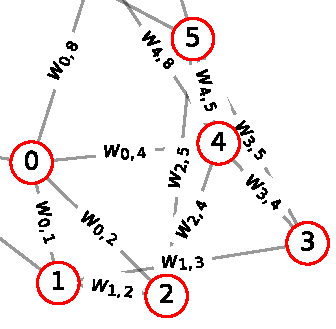
\includegraphics[width=\linewidth]{graph}
	\caption{Part of a small world network}
\end{figure}

\end{minipage}}
\only<2>{

Nonlinear $\Gamma$ must commute with $\e^{\I \zeta}$. (why?)
\vfill
We restrict ourselves to linear and nonlinear all-to-all coupling of the form
\[
\Gamma(\mathbf{z}) =zF(|z|)\qquad  \text{where}\qquad z = \frac{1}{n}\sum_{k=1}^nz_k.
\]
Assume $F:\reals_+ \rightarrow \complex$ is smooth, bounded and $F(|z|) \rightarrow 0$ as $|z|\rightarrow \infty$.
\vfill

For example: $\frac{1}{1+|z|^2}$, $\e^{-|z|}$ or Bessel functions $J_m(|z|)$ of the first kind.
}
\end{frame}
\begin{frame}{Coupled Limit Cycle Oscillators}
\[
 \quad \D{z_j}{t} = (\alpha - \beta|z_j|^2)z_j + \I\omega_jz_j +zF(|z|), \qquad j = 1,\ldots, n.
\]
with 
\[
z=\frac{1}{n}\sum_{k=1}^n z_k.
\]
\vfill

To recap:
\begin{itemize}
	\item Oscillators are modelled as points $z_j$ rotating in $\complex$,
	\item $\alpha, \beta$ are fixed parameters,
	\item $\omega_j$ is sampled from an \emph{even symmetric} distribution $g(\omega)$,  
	\item $F$ is smooth, bounded, and $F(|z|)\rightarrow 0$ as $|z|\rightarrow\infty$ ,
	\item The mean field $z$ is often a useful measure of coherence.
\end{itemize}
\vfill
\end{frame}
\section{Synch}
\subsection{Limit Cycle Dynamics}
\begin{frame}{Limit Cycle Dynamics}
\[
\quad \D{z_j}{t} = (\alpha - \beta|z_j|^2)z_j + \I\omega_jz_j +zF(|z|), \qquad j = 1,\ldots, n.
\]
\vfill
\begin{columns}
\begin{column}{.49\textwidth}
	\centering $\alpha <0$
	\begin{figure}
		\includegraphics[scale = 0.16]{node.png}
	\end{figure}
\end{column}
\begin{column}{.49\textwidth}
\begin{tcolorbox}[notitle, boxrule=1pt, colback=white]
	\centering
	$\alpha >0$
	\begin{figure}
		\includegraphics[scale = 0.16]{hopf.png}
	\end{figure}
\end{tcolorbox}
\end{column}
\end{columns}
\end{frame}
\begin{frame}{Deriving the Kuramoto Model}
\[
\quad \D{z_j}{t} = (\alpha - \beta|z_j|^2)z_j + \I\omega_jz_j +zF(|z|), \qquad j = 1,\ldots, n.
\]
Kuramoto~\cite{kuramoto75} considered the limit $\alpha, \beta \rightarrow \infty$ with $\alpha/\beta \rightarrow 1$, and $F(r)=K$ is real-valued and constant. \only<1>{Let $z_j=r_j\exp(\I\theta_j)$. It follows that 
\[
\frac{1}{z_j}\D{z_j}{t} = \D{\log z_j}{t}= \D{}{t}\left( \ln r_j + \I\theta_j\right) = \alpha -\beta r_j^2 + \I\omega_j + K\frac{r}{r_j}\e^{\I(\psi - \theta_j)}
\]
\begin{minipage}{0.6\linewidth}
we thus have
\begin{eqnarray*}
\frac{1}{\beta}\D{r_j}{t} &=& r_j(\frac{\alpha}{\beta} - r_j^2) + \frac{K}{\beta}\frac{r}{r_j}\cos(\psi-\theta_j)\\
\D{\theta_j}{t} &=&\omega_j + K\frac{r}{r_j}\sin(\psi-\theta_j)
\end{eqnarray*}
\end{minipage}\hfill
\begin{minipage}{0.275\linewidth}
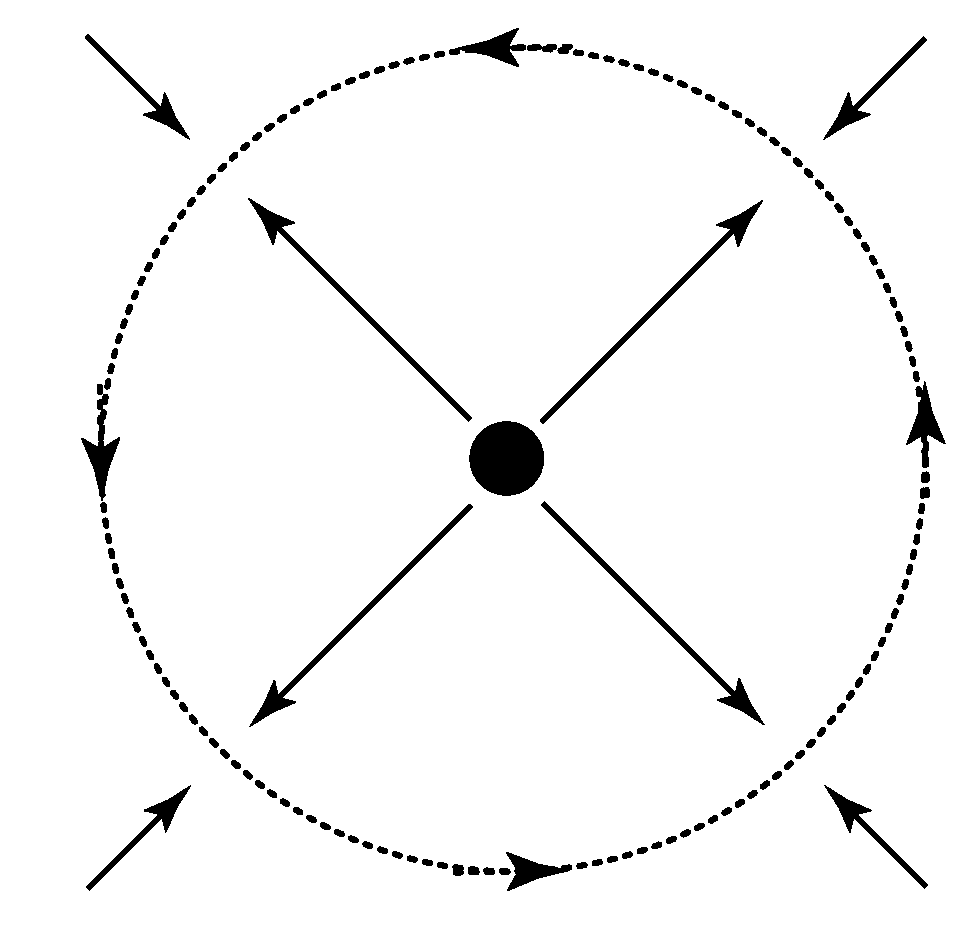
\includegraphics[height=0.3\textheight]{hopffast}
\end{minipage}
}
\only<2>{
\begin{minipage}{0.7\linewidth}
\vspace{10pt}

The system becomes a 'phase oscillator'
\[
\D{\theta_j}{t} = \omega_j + Kr\sin(\psi - \theta_j)
\]
\begin{itemize}
	\item The effective coupling strength is $Kr$!
	\item There is a Hopf at $K = 2/[\pi g(0)]$.
	\item When $K>K_c$, $r \rightarrow r_\infty$.
\end{itemize}
\end{minipage}\hfill
\begin{minipage}{0.3\linewidth}
	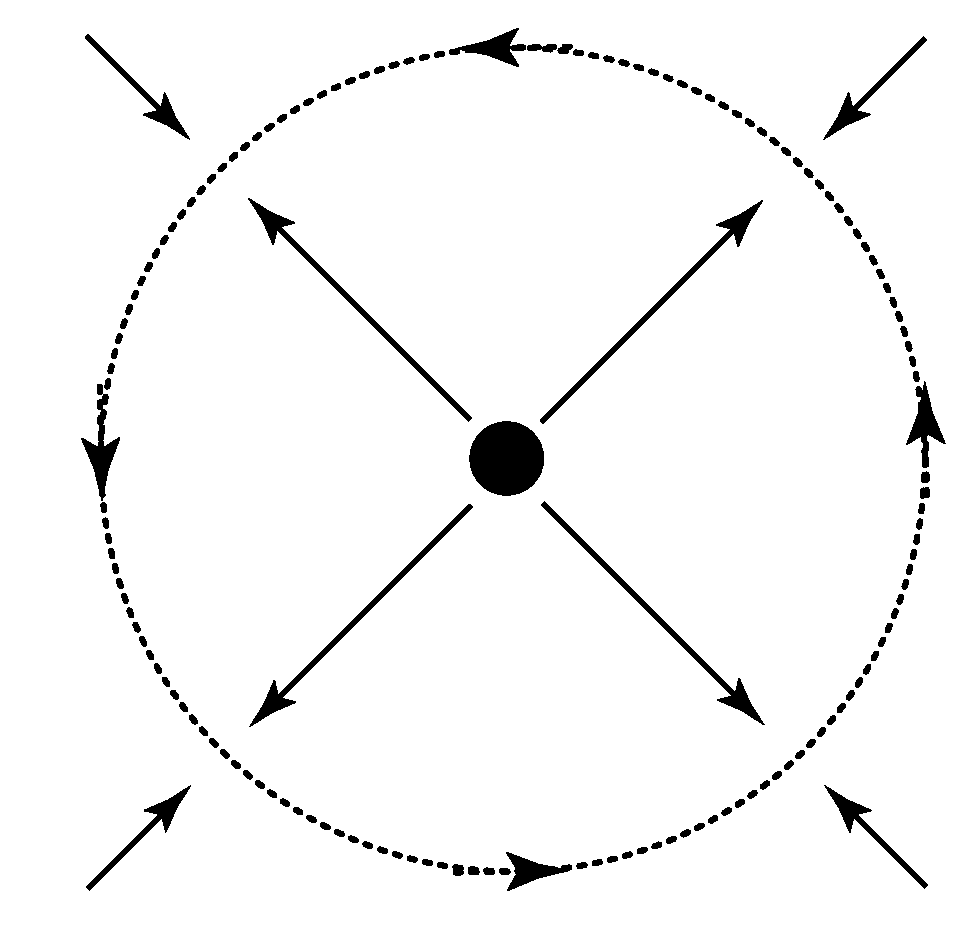
\includegraphics[height=0.3\textheight]{hopffast}
\end{minipage}


}
\end{frame}
\begin{frame}{Demonstration}
\centering
\vfill
...cut to Jupyter
\end{frame}
\begin{frame}{Amplitude Dynamics}
\[
\quad \D{z_j}{t} = (\alpha - \beta|z_j|^2)z_j + \I\omega_jz_j +zF(|z|), \qquad j = 1,\ldots, n.
\]
Matthews, Mirollo and Strogatz\cite{Matthews91} showed that in the $\alpha, \beta \approx O(1)$ regime there is a wide variety of dynamical states even for uni-modal $g$.
In addition to synchronised states and incoherence, they found:
\begin{itemize}
	\item amplitude death,
	\item quasi-periodic states,
	\item multi-stability,
	\item period doubling cascades and
	\item chaos
\end{itemize}
\end{frame}
\begin{frame}{Amplitude Death}
\[
\quad \D{z_j}{t} = (\alpha - \beta|z_j|^2)z_j + \I\omega_jz_j +zF(|z|), \qquad j = 1,\ldots, n.
\]

Amplitude death occurs when increasing the spread of frequencies causes the origin to become an attracting.
\vfill
Ermentrout\cite{Ermentrout90} showed that amplitude death 
\begin{itemize}
\item occurs in a wide variety of systems, 
\item does not depend special symmetries 
\item or infinite-range coupling
\end{itemize}
\end{frame}
\begin{frame}{Amplitude Death}
\[
\quad \D{z_j}{t} = (\alpha - \beta|z_j|^2)z_j + \I\omega_jz_j +zF(|z|), \qquad j = 1,\ldots, n.
\]
Mirollo and Strogatz~\cite{Mirollo90} defined
$f(\mu) = \int_{-\infty}^\infty \frac{g(\omega)}{\mu - \I\omega}\df{\omega}$
\begin{tcolorbox}[notitle, boxrule=0pt, colback=lred]
\begin{theorem}[\citeauthor{Mirollo90}]
Let $\alpha = 1-K$, $F(|z|)=K$ and assume that the density $g(\omega)$ is an even function which is nonincreasing on $[0,\infty)$.
Then: 
\begin{itemize}
	\item (A) Amplitude death is stable with 
	probability $\rightarrow 1$ as $n \rightarrow \infty$, $f(K-1) < \frac{1}{K}$
\item (B) Amplitude death is stable with 
probability $\rightarrow 1$ as $n \rightarrow \infty$, $f(K-1) > \frac{1}{K}$
\end{itemize}
\end{theorem}
\end{tcolorbox}
\end{frame}
\begin{frame}{Demonstration of amplitude death.}
\centering
\vfill
...some more examples.
\end{frame}
\begin{frame}{The Dispersion Function}
\[
\quad \D{z_j}{t} = (\alpha - \beta|z_j|^2)z_j + \I\omega_jz_j +zF(|z|), \qquad j = 1,\ldots, n.
\]
Matthews, Mirollo and Strogatz~\cite{Matthews91} considered the dispersion function
\[f(\mu) = \int_{-\infty}^\infty \frac{g(\omega)}{\mu - \I\omega}\df{\omega}.\]
for real valued $\mu$.

When $g$ is symmetric and unimodal
\begin{itemize}
\item $f(\mu)$ is real valued iff $\mu$ real valued.
\item $f$ is odd and strictly decreasing on $[0,\infty)$
\item $f$ is discontinuous at $\mu=0$ and $\lim_{\mu\rightarrow 0^+} = \pi g(0)$.
\end{itemize}
\end{frame}
\subsection{Stable Node Dynamics}
\begin{frame}{Stable Node Dynamics}
\[
\quad \D{z_j}{t} = (\alpha - \beta|z_j|^2)z_j + \I\omega_jz_j +zF(|z|), \qquad j = 1,\ldots, n.
\]
\vfill
\begin{columns}
	\begin{column}{.49\textwidth}
				\begin{tcolorbox}[notitle, boxrule=1pt, colback=white]
		\centering $\alpha <0$
		\begin{figure}
			\includegraphics[scale = 0.16]{node.png}
		\end{figure}
			\end{tcolorbox}
	\end{column}
	\begin{column}{.49\textwidth}
			\centering
			$\alpha >0$
			\begin{figure}
				\includegraphics[scale = 0.16]{hopf.png}
			\end{figure}
	\end{column}
\end{columns}
\end{frame}
\begin{frame}{Amplitude Death}
\[
\D{z_j}{t} = (\alpha - \beta|z_j|^2)z_j + \I\omega_jz_j +zF(|z|), \qquad j = 1,\ldots, n.
\]
Consider the case where $\alpha = -1$,$\beta=0$, $F$ smooth, bounded and $F\rightarrow 0$ as $|z|\rightarrow\infty$.  
\vfill
\only<1>{
	It follows from a fixed point argument that amplitude death and full synchronisation are the only limiting sets.
\vspace{10pt}
In particular, $z_j$ is fixed iff $z$ is fixed up to a constant $\exp(\I\Omega t + \Theta_0)$}
\only<2>{
\begin{tcolorbox}[notitle, boxrule=0pt, colback=lred]
\begin{theorem}[\citeauthor{pc2015}]
	Let $g$ be a even symmetric probability distribution, non-increasing on $[0,\infty)$, let $A = \{\lambda: \Re[\lambda] > 1\} \subset\complex$ and $E = 1/f(A)\subset\complex$. Then amplitude death is unstable with probability $\rightarrow 1$ as $n\rightarrow \infty$ if and only if $F(0) \in E$.
\end{theorem}
\end{tcolorbox}
}
\end{frame}
\begin{frame}{Demonstration of Amplitude Death.}
\centering
\vfill
...more Jupyter Examples.
\end{frame}
\begin{frame}{Proof of Amplitude Death}
\only<1>{
To prove the stability result we require:
\begin{tcolorbox}[notitle, boxrule=0pt, colback=lred]
\begin{theorem}{\citeauthor{pc2015}}
	Let $g(\omega)$ be an even symmetric probability distribution, non-increasing on $[0,\infty)$. Then the dispersion function $f: \complex_+\rightarrow Y \subset\complex_+$ is bijective and holomorphic.
\end{theorem}
\end{tcolorbox}
}
\only<2>{
Sketch of the proof:
\begin{itemize}
	\item Linearise the system about $z_j=0$..
	\item Show that the limiting operator has has continuous spectrum along $\Re[\lambda] = -1$, and a discrete spectrum at $F(0) = \frac{1}{f(\lambda+1)}$.
	\item Use the conformal property of $f$ to show $F(0)\in E$ implies $\lambda+1 \in A$ and hence fixed point is unstable.
\end{itemize}}
\begin{center}
	\includegraphics[scale=0.8]{scm2}
\end{center}	
\end{frame}
\begin{frame}{Synchronised States}
\[
\D{z_j}{t} = (\alpha - \beta|z_j|^2)z_j + \I\omega_jz_j +zF(|z|), \qquad j = 1,\ldots, n.
\]
Consider the case where $\alpha = -1$,$\beta=0$, $F$ smooth, bounded and $F\rightarrow 0$ as $|z|\rightarrow\infty$.  
\vfill
There are also results on stability and bifurcations\cite{pc2015} which are expressed in terms of a playoff between
\begin{itemize}
	\item Population heterogeneity (via $f(\mu) = \int_{-\infty}^\infty \frac{g(\omega)}{\mu - \I\omega}\df{\omega}$ and it's derivatives) and 
	\item coupled topology (via the `shape' of $F$)
\end{itemize}
\end{frame}
\section{Conclusion}
\begin{frame}{In Summary}
Hopefully i've convinced you that:
\begin{itemize}
	\item Synchronisation is an example of emergence,
	\item resulting from mutual interactions between parts of a larger system.
	\item The different coupling mechanisms and population variability can lead to differing synchronisation properties,
	\item which can be simulated and, in some cases, solved explicitly.
	\item There are also deep mathematical properties buried not far from the surface.
\end{itemize}
\end{frame}
\begin{frame}{Thanks and Acknowledgements}
Thanks to 
\begin{itemize}
	\item Dr. Stuart Johnson and the MCB seminar organisers.
	\item Prof. Edmund Crampin and The Systems Biology Laboratory.
\end{itemize}

This research was performed under the supervision of Dr. Catherine. A. Holmes, Prof. Joseph Grotowski and Dr. Cecilia Gonzales Tokman at the University of Queensland (UQ) as part the doctoral program funded by the ARC.
\vspace{12pt}

Additional thanks to Prof. Gerard Milburn, Dr. James Bennett at the UQ ARC Centre of Excellence for Engineered Quantum Systems (EQUS).
\end{frame}
\subsection{Appendices and References}
\begin{frame}{Appendix: Quantum Optomechanics}
\begin{figure}
\includegraphics[width=0.9\linewidth]{cavity.jpg}\caption{An optomechanical system~\cite{nanoimg}}
\end{figure}
\end{frame}
\begin{frame}{Appendix: Schematic of an optomechanical system}
\begin{figure}
	\includegraphics[width=0.9\linewidth]{schem2}\caption{Optomechanical equivalent circuit}
\end{figure}
\end{frame}
\begin{frame}[allowframebreaks]
\frametitle{References}
\tiny
\printbibliography
\end{frame}
\end{document}